\documentclass{standalone}

\usepackage[T1]{fontenc}
\usepackage[utf8]{inputenc}
\usepackage{eulervm}
\usepackage{amsmath}
\usepackage{bm}
\usepackage{tikz}
\usepackage{environ}

\usetikzlibrary{fit}
\usetikzlibrary{patterns}
\usetikzlibrary{arrows}
\usetikzlibrary{positioning}

\input{colors}

\begin{document}
  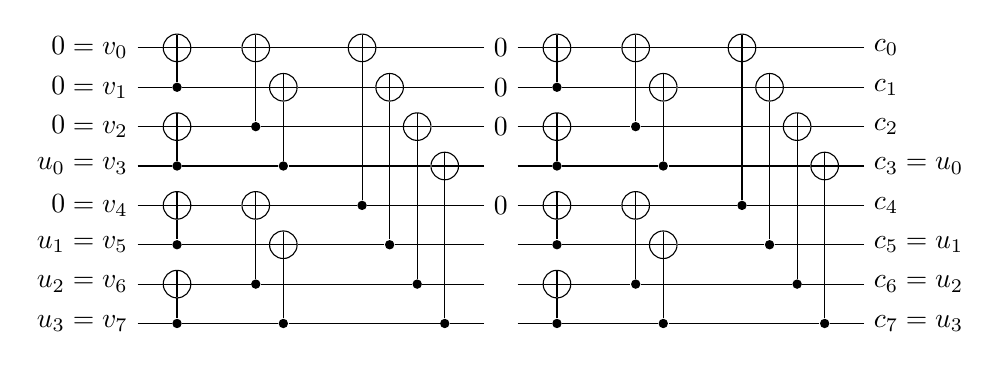
\begin{tikzpicture}%[scale=\tikzscale]

  \tikzset{XOR/.style={draw,circle, minimum height=0.35cm,append after command={
          [shorten >=\pgflinewidth, shorten <=\pgflinewidth,]
          (\tikzlastnode.north) edge (\tikzlastnode.south)
          (\tikzlastnode.east) edge (\tikzlastnode.west)
          }
      }
  }

  \tikzset{DOT/.style={circle,fill,inner sep=1.2pt} }

  \newcommand\startx{0.0}
  \newcommand\startyg{0}
  \newcommand\sed{0.50}
  \newcommand\stasep{1.00}
  \newcommand\xorsep{0.35}

  \renewcommand\startyg{0.0}


  \node[XOR] (g3_x0) at (\startx,                 \startyg+1.75)       {};
  \node      (g3_e0) at (\startx,                 \startyg+1.25) [DOT] {};

  \node[XOR] (g3_x1) at (\startx,                 \startyg+0.75)       {};
  \node      (g3_e1) at (\startx,                 \startyg+0.25) [DOT] {};

  % ---

  \node[XOR] (g3_x2) at (\startx+\stasep,         \startyg+1.75)       {};
  \node[XOR] (g3_x3) at (\startx+\stasep+\xorsep, \startyg+1.25)       {};

  \node      (g3_e2) at (\startx+\stasep,         \startyg+0.75) [DOT] {};
  \node      (g3_e3) at (\startx+\stasep+\xorsep, \startyg+0.25) [DOT] {};

  % -----

  \node[XOR] (g3_x4) at (\startx,                 \startyg-0.25)       {};
  \node      (g3_e4) at (\startx,                 \startyg-0.75) [DOT] {};

  \node[XOR] (g3_x5) at (\startx,                 \startyg-1.25)       {};
  \node      (g3_e5) at (\startx,                 \startyg-1.75) [DOT] {};

  % ---

  \node[XOR] (g3_x6) at (\startx+\stasep,         \startyg-0.25)       {};
  \node[XOR] (g3_x7) at (\startx+\stasep+\xorsep, \startyg-0.75)       {};

  \node      (g3_e6) at (\startx+\stasep,         \startyg-1.25) [DOT] {};
  \node      (g3_e7) at (\startx+\stasep+\xorsep, \startyg-1.75) [DOT] {};

  % ----------

  \node[XOR] (g3_x8)  at (\startx+\stasep+\stasep+\xorsep,                         \startyg+1.75)       {};
  \node[XOR] (g3_x9)  at (\startx+\stasep+\stasep+\xorsep+\xorsep,                 \startyg+1.25)       {};
  \node[XOR] (g3_x10) at (\startx+\stasep+\stasep+\xorsep+\xorsep+\xorsep,         \startyg+0.75)       {};
  \node[XOR] (g3_x11) at (\startx+\stasep+\stasep+\xorsep+\xorsep+\xorsep+\xorsep, \startyg+0.25)       {};

  \node      (g3_e8)  at (\startx+\stasep+\stasep+\xorsep,                         \startyg-0.25) [DOT] {};
  \node      (g3_e9)  at (\startx+\stasep+\stasep+\xorsep+\xorsep,                 \startyg-0.75) [DOT] {};
  \node      (g3_e10) at (\startx+\stasep+\stasep+\xorsep+\xorsep+\xorsep,         \startyg-1.25) [DOT] {};
  \node      (g3_e11) at (\startx+\stasep+\stasep+\xorsep+\xorsep+\xorsep+\xorsep, \startyg-1.75) [DOT] {};

  \draw[-,>=latex] (\startx-\sed, \startyg+1.75) node[left] {$0 = v_0$} -- (g3_x0);
  \draw[-,>=latex] (\startx-\sed, \startyg+1.25) node[left] {$0 = v_1$} -- (g3_e0);
  \draw[-,>=latex] (g3_x0)                       -- (g3_e0);
  \draw[-,>=latex] (g3_x0)                       -- (g3_x2);
  \draw[-,>=latex] (g3_e0)                       -- (g3_x3);

  \draw[-,>=latex] (\startx-\sed, \startyg+0.75) node[left] {$0 = v_2$} -- (g3_x1);
  \draw[-,>=latex] (\startx-\sed, \startyg+0.25) node[left] {$u_0 = v_3$} -- (g3_e1);
  \draw[-,>=latex] (g3_x1)                       -- (g3_e1);
  \draw[-,>=latex] (g3_x1)                       -- (g3_e2);
  \draw[-,>=latex] (g3_e1)                       -- (g3_e3);
  \draw[-,>=latex] (g3_e2)                       -- (g3_x2);
  \draw[-,>=latex] (g3_e3)                       -- (g3_x3);
  \draw[-,>=latex] (g3_x2)                       -- (g3_x8);
  \draw[-,>=latex] (g3_x3)                       -- (g3_x9);
  \draw[-,>=latex] (g3_e2)                       -- (g3_x10);
  \draw[-,>=latex] (g3_e3)                       -- (g3_x11);

  \draw[-,>=latex] (\startx-\sed, \startyg-0.25) node[left] {$0 = v_4$} -- (g3_x4);
  \draw[-,>=latex] (\startx-\sed, \startyg-0.75) node[left] {$u_1 = v_5$} -- (g3_e4);
  \draw[-,>=latex] (g3_x4)                       -- (g3_e4);
  \draw[-,>=latex] (g3_x4)                       -- (g3_x6);
  \draw[-,>=latex] (g3_e4)                       -- (g3_x7);

  \draw[-,>=latex] (\startx-\sed, \startyg-1.25) node[left] {$u_2 = v_6$} -- (g3_x5);
  \draw[-,>=latex] (\startx-\sed, \startyg-1.75) node[left] {$u_3 = v_7$} -- (g3_e5);
  \draw[-,>=latex] (g3_x5)                       -- (g3_e5);
  \draw[-,>=latex] (g3_x5)                       -- (g3_e6);
  \draw[-,>=latex] (g3_e5)                       -- (g3_e7);
  \draw[-,>=latex] (g3_e6)                       -- (g3_x6);
  \draw[-,>=latex] (g3_e7)                       -- (g3_x7);
  \draw[-,>=latex] (g3_x6)                       -- (g3_e8);
  \draw[-,>=latex] (g3_x7)                       -- (g3_e9);
  \draw[-,>=latex] (g3_e6)                       -- (g3_e10);
  \draw[-,>=latex] (g3_e7)                       -- (g3_e11);

  \draw [-,>=latex] (g3_e8)                      -- (g3_x8);
  \draw [-,>=latex] (g3_e9)                      -- (g3_x9);
  \draw [-,>=latex] (g3_e10)                     -- (g3_x10);
  \draw [-,>=latex] (g3_e11)                     -- (g3_x11);

  % \draw[-,>=latex] (\startx+\stasep+\stasep+\xorsep+\xorsep+\xorsep+\sed, \startyg+1.75) node[right] {$c_0 = v_0 \oplus v_1 \oplus v_2 \oplus v_3 \oplus v_4 \oplus v_5 \oplus v_6 \oplus v_7$} -- (g3_x8);
  \draw[-,>=latex] (\startx+\stasep+\stasep+\xorsep+\xorsep+\xorsep+\xorsep+\sed, \startyg+1.75) node[right] {$0$} -- (g3_x8);
  \draw[-,>=latex] (\startx+\stasep+\stasep+\xorsep+\xorsep+\xorsep+\xorsep+\sed, \startyg+1.25) node[right] {$0$} -- (g3_x9);
  \draw[-,>=latex] (\startx+\stasep+\stasep+\xorsep+\xorsep+\xorsep+\xorsep+\sed, \startyg+0.75) node[right] {$0$} -- (g3_x10);
  \draw[-,>=latex] (\startx+\stasep+\stasep+\xorsep+\xorsep+\xorsep+\xorsep+\sed, \startyg+0.25) node[right] {   } -- (g3_x11);
  \draw[-,>=latex] (\startx+\stasep+\stasep+\xorsep+\xorsep+\xorsep+\xorsep+\sed, \startyg-0.25) node[right] {$0$} -- (g3_e8);
  \draw[-,>=latex] (\startx+\stasep+\stasep+\xorsep+\xorsep+\xorsep+\xorsep+\sed, \startyg-0.75) node[right] {   } -- (g3_e9);
  \draw[-,>=latex] (\startx+\stasep+\stasep+\xorsep+\xorsep+\xorsep+\xorsep+\sed, \startyg-1.25) node[right] {   } -- (g3_e10);
  \draw[-,>=latex] (\startx+\stasep+\stasep+\xorsep+\xorsep+\xorsep+\xorsep+\sed, \startyg-1.75) node[right] {   } -- (g3_e11);

  % \node[draw=Paired-1, scale=0.95, rounded corners=2pt, dashed, fit=(g3_x0) (g3_e0)] (g3_l3_1) {};
  % \node[draw=Paired-1, scale=0.95, rounded corners=2pt, dashed, fit=(g3_x1) (g3_e1)] (g2_l3_2) {};
  % \node[draw=Paired-1, scale=0.95, rounded corners=2pt, dashed, fit=(g3_x4) (g3_e4)] (g3_l3_3) {};
  % \node[draw=Paired-1, scale=0.95, rounded corners=2pt, dashed, fit=(g3_x5) (g3_e5)] (g2_l3_4) {};

  % \node[draw=Paired-3, scale=0.975, rounded corners=2pt, dashed, fit=(g3_x2) (g3_x3) (g3_e2) (g3_e3)] (g3_l1_1) {};
  % \node[draw=Paired-3, scale=0.975, rounded corners=2pt, dashed, fit=(g3_x6) (g3_x7) (g3_e6) (g3_e7)] (g3_l1_2) {};

  % \node[draw=Paired-5, scale=0.987, rounded corners=2pt, dashed, fit=(g3_x8) (g3_x11) (g3_e8) (g3_e11)] (g3_l1_1) {};


  % ---------------------------------------------------------------------------
  % ---------------------------------------------------------------------------
  % ---------------------------------------------------------------------------

  \renewcommand\startx{4.825}

  \node[XOR] (g3_x0) at (\startx,                 \startyg+1.75)       {};
  \node      (g3_e0) at (\startx,                 \startyg+1.25) [DOT] {};

  \node[XOR] (g3_x1) at (\startx,                 \startyg+0.75)       {};
  \node      (g3_e1) at (\startx,                 \startyg+0.25) [DOT] {};

  % ---

  \node[XOR] (g3_x2) at (\startx+\stasep,         \startyg+1.75)       {};
  \node[XOR] (g3_x3) at (\startx+\stasep+\xorsep, \startyg+1.25)       {};

  \node      (g3_e2) at (\startx+\stasep,         \startyg+0.75) [DOT] {};
  \node      (g3_e3) at (\startx+\stasep+\xorsep, \startyg+0.25) [DOT] {};

  % -----

  \node[XOR] (g3_x4) at (\startx,                 \startyg-0.25)       {};
  \node      (g3_e4) at (\startx,                 \startyg-0.75) [DOT] {};

  \node[XOR] (g3_x5) at (\startx,                 \startyg-1.25)       {};
  \node      (g3_e5) at (\startx,                 \startyg-1.75) [DOT] {};

  % ---

  \node[XOR] (g3_x6) at (\startx+\stasep,         \startyg-0.25)       {};
  \node[XOR] (g3_x7) at (\startx+\stasep+\xorsep, \startyg-0.75)       {};

  \node      (g3_e6) at (\startx+\stasep,         \startyg-1.25) [DOT] {};
  \node      (g3_e7) at (\startx+\stasep+\xorsep, \startyg-1.75) [DOT] {};

  % ----------

  \node[XOR] (g3_x8)  at (\startx+\stasep+\stasep+\xorsep,                         \startyg+1.75)       {};
  \node[XOR] (g3_x9)  at (\startx+\stasep+\stasep+\xorsep+\xorsep,                 \startyg+1.25)       {};
  \node[XOR] (g3_x10) at (\startx+\stasep+\stasep+\xorsep+\xorsep+\xorsep,         \startyg+0.75)       {};
  \node[XOR] (g3_x11) at (\startx+\stasep+\stasep+\xorsep+\xorsep+\xorsep+\xorsep, \startyg+0.25)       {};

  \node      (g3_e8)  at (\startx+\stasep+\stasep+\xorsep,                         \startyg-0.25) [DOT] {};
  \node      (g3_e9)  at (\startx+\stasep+\stasep+\xorsep+\xorsep,                 \startyg-0.75) [DOT] {};
  \node      (g3_e10) at (\startx+\stasep+\stasep+\xorsep+\xorsep+\xorsep,         \startyg-1.25) [DOT] {};
  \node      (g3_e11) at (\startx+\stasep+\stasep+\xorsep+\xorsep+\xorsep+\xorsep, \startyg-1.75) [DOT] {};

  \draw[-,>=latex] (\startx-\sed, \startyg+1.75) -- (g3_x0);
  \draw[-,>=latex] (\startx-\sed, \startyg+1.25) -- (g3_e0);
  \draw[-,>=latex] (g3_x0)                       -- (g3_e0);
  \draw[-,>=latex] (g3_x0)                       -- (g3_x2);
  \draw[-,>=latex] (g3_e0)                       -- (g3_x3);

  \draw[-,>=latex] (\startx-\sed, \startyg+0.75) -- (g3_x1);
  \draw[-,>=latex] (\startx-\sed, \startyg+0.25) -- (g3_e1);
  \draw[-,>=latex] (g3_x1)                       -- (g3_e1);
  \draw[-,>=latex] (g3_x1)                       -- (g3_e2);
  \draw[-,>=latex] (g3_e1)                       -- (g3_e3);
  \draw[-,>=latex] (g3_e2)                       -- (g3_x2);
  \draw[-,>=latex] (g3_e3)                       -- (g3_x3);
  \draw[-,>=latex] (g3_x2)                       -- (g3_x8);
  \draw[-,>=latex] (g3_x3)                       -- (g3_x9);
  \draw[-,>=latex] (g3_e2)                       -- (g3_x10);
  \draw[-,>=latex] (g3_e3)                       -- (g3_x11);

  \draw[-,>=latex] (\startx-\sed, \startyg-0.25) -- (g3_x4);
  \draw[-,>=latex] (\startx-\sed, \startyg-0.75) -- (g3_e4);
  \draw[-,>=latex] (g3_x4)                       -- (g3_e4);
  \draw[-,>=latex] (g3_x4)                       -- (g3_x6);
  \draw[-,>=latex] (g3_e4)                       -- (g3_x7);

  \draw[-,>=latex] (\startx-\sed, \startyg-1.25) -- (g3_x5);
  \draw[-,>=latex] (\startx-\sed, \startyg-1.75) -- (g3_e5);
  \draw[-,>=latex] (g3_x5)                       -- (g3_e5);
  \draw[-,>=latex] (g3_x5)                       -- (g3_e6);
  \draw[-,>=latex] (g3_e5)                       -- (g3_e7);
  \draw[-,>=latex] (g3_e6)                       -- (g3_x6);
  \draw[-,>=latex] (g3_e7)                       -- (g3_x7);
  \draw[-,>=latex] (g3_x6)                       -- (g3_e8);
  \draw[-,>=latex] (g3_x7)                       -- (g3_e9);
  \draw[-,>=latex] (g3_e6)                       -- (g3_e10);
  \draw[-,>=latex] (g3_e7)                       -- (g3_e11);

  \draw [-,>=latex] (g3_e8)                      -- (g3_x8);
  \draw [-,>=latex] (g3_e9)                      -- (g3_x9);
  \draw [-,>=latex] (g3_e10)                     -- (g3_x10);
  \draw [-,>=latex] (g3_e11)                     -- (g3_x11);

  % \draw[-,>=latex] (\startx+\stasep+\stasep+\xorsep+\xorsep+\xorsep+\sed, \startyg+1.75) node[right] {$c_0 = v_0 \oplus v_1 \oplus v_2 \oplus v_3 \oplus v_4 \oplus v_5 \oplus v_6 \oplus v_7$} -- (g3_x8);
  \draw[-,>=latex] (\startx+\stasep+\stasep+\xorsep+\xorsep+\xorsep+\xorsep+\sed, \startyg+1.75) node[right] {$c_0$}       -- (g3_x8);
  \draw[-,>=latex] (\startx+\stasep+\stasep+\xorsep+\xorsep+\xorsep+\xorsep+\sed, \startyg+1.25) node[right] {$c_1$}       -- (g3_x9);
  \draw[-,>=latex] (\startx+\stasep+\stasep+\xorsep+\xorsep+\xorsep+\xorsep+\sed, \startyg+0.75) node[right] {$c_2$}       -- (g3_x10);
  \draw[-,>=latex] (\startx+\stasep+\stasep+\xorsep+\xorsep+\xorsep+\xorsep+\sed, \startyg+0.25) node[right] {$c_3 = u_0$} -- (g3_x11);
  \draw[-,>=latex] (\startx+\stasep+\stasep+\xorsep+\xorsep+\xorsep+\xorsep+\sed, \startyg-0.25) node[right] {$c_4$}       -- (g3_e8);
  \draw[-,>=latex] (\startx+\stasep+\stasep+\xorsep+\xorsep+\xorsep+\xorsep+\sed, \startyg-0.75) node[right] {$c_5 = u_1$} -- (g3_e9);
  \draw[-,>=latex] (\startx+\stasep+\stasep+\xorsep+\xorsep+\xorsep+\xorsep+\sed, \startyg-1.25) node[right] {$c_6 = u_2$} -- (g3_e10);
  \draw[-,>=latex] (\startx+\stasep+\stasep+\xorsep+\xorsep+\xorsep+\xorsep+\sed, \startyg-1.75) node[right] {$c_7 = u_3$} -- (g3_e11);

  % \node[draw=Paired-1, scale=0.95, rounded corners=2pt, dashed, fit=(g3_x0) (g3_e0)] (g3_l3_1) {};
  % \node[draw=Paired-1, scale=0.95, rounded corners=2pt, dashed, fit=(g3_x1) (g3_e1)] (g2_l3_2) {};
  % \node[draw=Paired-1, scale=0.95, rounded corners=2pt, dashed, fit=(g3_x4) (g3_e4)] (g3_l3_3) {};
  % \node[draw=Paired-1, scale=0.95, rounded corners=2pt, dashed, fit=(g3_x5) (g3_e5)] (g2_l3_4) {};

  % \node[draw=Paired-3, scale=0.975, rounded corners=2pt, dashed, fit=(g3_x2) (g3_x3) (g3_e2) (g3_e3)] (g3_l1_1) {};
  % \node[draw=Paired-3, scale=0.975, rounded corners=2pt, dashed, fit=(g3_x6) (g3_x7) (g3_e6) (g3_e7)] (g3_l1_2) {};

  % \node[draw=Paired-5, scale=0.987, rounded corners=2pt, dashed, fit=(g3_x8) (g3_x11) (g3_e8) (g3_e11)] (g3_l1_1) {};







  \end{tikzpicture}
\end{document}